\newpage

\paragraph{\LARGE Aufgabe 7 - Verzeichnisse}

\section{Aufgabenstellung}
	\subsection{Aufgabe 1: Typische Verzeichnisstrukturen}
		\begin{quote}
			\begin{itemize}
				\item Geben Sie die typische Verzeichnisstruktur einer aktuellen Linuxdistribution an. Was ist in den Verzeichnissen enthalten? Nennen Sie mindenstens f\"unf Beispiele (wie /etc, /usr usw.). Finden Sie zus\"atzlich heraus, wo Log-Dateien gespeichert werden. Wo liegen ausgelagerte Inhalte des Hauptspeichers?\\
				\item Geben Sie die typische Ordnerstruktur von Microsoft Windows an. Nennen Sie analog zur vor vorherigen Aufgabe einige beispielhafte Inhalte der jeweiligen Verzeichnisse (wie z.B, C:\textbackslash Windows\textbackslash System32).\\
			\end{itemize}
		\end{quote}
	\subsection{Aufgabe 2: Verzeichnisse}
		\begin{quote}
			Entwickeln Sie ein Programm myls, das den Inhalt von Verzeichnissen ausgibt. Die grundlegende Funktion ist in etwa vergleichbar mit dem Shell-Kommando ls.\\ \\
			Randbedingungen: \\
			\begin{itemize}
				\item Der Name des auszulesenden Verzeichnisses soll dem Programm als Argument \"ubergeben werden. Wird kein Verzeichnis angegeben, so wird das lokale Verzeichnis ausgegeben.\\
				\item Sie sollen die Funktionen opendir(), readdir() und closedir() verwenden, um die Eintr\"age des Verzeichnisses abzufragen.\\
				\item F\"ur den Zugriff auf Informationen zu den Eintr\"agen kann die Funktion lstat() verwendet werden. Diese lifert deterillierte Informationen zu jedem Verzeichniseintrag. Sie sollen mindestens die Attribute abragen und ausgeben, die bei Eingabe des Befehls ls -algo auf UNIX / Linux-System ausgegeben werden.\\
				\item Ihr Programm soll hinsichtlich der beiden Optionen -a und -l parametrisierbar sein die beiden Parameter k\"onnen auch zusammen angewendet werden, also myls -a -l oder myls -al. Hinsichtlich der Bedeutung der Parameter k\"onnen Sie sich an dem Standard-UNIX/Linux-Kommando orientieren.\\
				\item Verwenden Sie getopt(), um die Ausgabeparameter von der Kommandozeile einzulesen.\\
				\item Ihr Programm braucht keine weiteren Argumente oder Parameter zu unterst\"utzen.\\
				\item Geben Sie bei gesetzter Option -l den Namen ausf\"uhrbarer Dareien in rot und den Namen von C-Dateien (Dateiendung: .c) in gr\"un aus. Nutzen Sie f\"ur die Einf\"arbung von Verzeichniseintr\"agen Escape Sequenzen, die Sie beispielsweise unter http://www.linupedia.org/opensuse/Farbe\_in\_der\_Konsole finden.\\
			\end{itemize}
		\end{quote}
\newpage
\section{Aufgabe 7.1}
	\subsection{Vorbereitung}
		\begin{quote}
			Den Eintrag Verzeichsstuktur aus \\ ''https://wiki.ubuntuusers.de/Verzeichnisstruktur/'' lesen\\
		\end{quote}
	\subsection{Durchführung}
		\begin{quote}
			Ergebnisse recherchieren und protokollieren.\\
		\end{quote}
	\subsection{Fazit}
		\begin{quote}
			Aufgabe 7.1.1\\ \\
			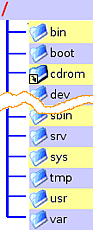
\includegraphics[width=2.0cm]{images/linux_verzeichnisstruktur}
			/bin:\\
			Enth\"alt f\"ur Linux unverzichtbare Programme.\\ \\
			/boot:\\
			Enth\"alt zum Booten benötigte Dateien.\\ \\
			/dev:\\
			Enth\"alt alle Gerätedateien, \"uber die die Hardware im Betrieb angesprochen wird.\\ \\
			/etc:\\
			Enth\"alt Konfigurations- und Informationsdateien des Basissystems.\\ \\
			/lib:\\
			Enth\"alt unverzichtbare Bibliotheken fürs Booten und die dynamisch gelinkten Programme des Basissystems.\\ \\
			/var/log:\\
			Enth\"alt alle Log-Dateien der Systemprogramme.\\ \\
			/var/cache ist vorgesehen als Datenpuffer für Anwendungsproramme.\\ \\ \\
			Aufgabe 7.1.2\\ \\
			C:\textbackslash Users:\\
			Enth\"alt Verzeichnisse der Benutzer.\\ \\
			C:\textbackslash Files:\\
			Enth\"alt  installierte Programme.\\ \\
			C:\textbackslash Temp:\\
			Enth\"alt  tempor\"are Dateien.\\ \\
			C:\textbackslash Windows\textbackslash Help:\\
			Enth\"alt  Hilfe-Dateien.\\ \\
			C:\textbackslash Windows\textbackslash Fonts:\\
			Enth\"alt  Schrifttyp-Dateien\\ \\
			C:\textbackslash Windows\textbackslash Logs:\\
			Enth\"alt alle Log-Dateien der Systemprogramme.\\ \\
			C:\textbackslash pagefile.sys:\\
			Speichert ausgelagerte Inhalte des Hauptspeichers.\\ \\
		\end{quote}

\section{Aufgabe 7.2}
	\subsection{Vorbereitung}
		\begin{quote}
			C-Projekt anlegen.\\
			Makefile schreiben.\\
		\end{quote}
	\subsection{Durchführung}
		\begin{quote}
			Code schreiben und dann testen bzw debuggen.\\
		\end{quote}
	\subsection{Fazit}
		\begin{quote}
			
		\end{quote}